\documentclass[a4paper,12pt]{article}

% ----- بسته‌های مورد نیاز -----
\usepackage{amsmath, amsthm, amssymb} % برای فرمول‌های ریاضی
\usepackage{graphicx} % برای قرار دادن تصاویر و نمودارها
\usepackage{float} % برای تنظیم دقیق مکان عکس‌ها
\usepackage[hidelinks]{hyperref} % برای لینک دادن (مثل لینک گیت‌هاب)
\usepackage{geometry} % برای تنظیم حاشیه‌های صفحه
\geometry{top=2.5cm, bottom=2.5cm, left=2.5cm, right=2.5cm}

\usepackage{xcolor}
\usepackage{listings} % برای قرار دادن کدهای پایتون

% تنظیمات پکیج listings برای نمایش بهینه کدهای پایتون
\lstset{
    language=Python,
    basicstyle=\ttfamily\small,
    keywordstyle=\color{blue}\bfseries,
    stringstyle=\color{purple},
    commentstyle=\color{gray}\itshape,
    numbers=left,
    numberstyle=\tiny\color{gray},
    stepnumber=1,
    breaklines=true,
    frame=single,
    showstringspaces=false,
    tabsize=4
}

% بسته زی‌پرشین برای پشتیبانی از زبان فارسی (باید آخرین بسته باشد)
\usepackage{xepersian}
\settextfont{B Nazanin} % فونت متن اصلی

\title{\textbf{گزارش پروژه ۳ - نرم افزار ریاضی}}
\author{سعد ملائی \and شماره دانشجویی: 40113027}
\date{تیر 1405}

\begin{document}

\maketitle

% ==========================================
\section{درون‌یابی لاگرانژ و اسپلاین مکعبی}
در این بخش، هدف درون‌یابی نقاط داده شده زیر با استفاده از دو روش چندجمله‌ای لاگرانژ و اسپلاین مکعبی است:
\[ \{(1,1), (2,3), (3,5), (4,8), (5,5), (6,2)\} \]

\subsection{کد پایتون پیاده‌سازی}
برای محاسبات نمادین و استخراج ضابطه دقیق از کتابخانه \texttt{SymPy} و برای محاسبه ضرایب اسپلاین از کتابخانه \texttt{SciPy} استفاده شده است:

\begin{latin}
\begin{lstlisting}[language=Python]
import numpy as np
import sympy as sp
from scipy.interpolate import CubicSpline

x_vals = np.array([1, 2, 3, 4, 5, 6])
y_vals = np.array([1, 3, 5, 8, 5, 2])
x = sp.Symbol('x')

# 1. Lagrange Interpolation
lagrange_poly = 0
for i in range(len(x_vals)):
    term = y_vals[i]
    for j in range(len(x_vals)):
        if i != j:
            term *= (x - x_vals[j]) / (x_vals[i] - x_vals[j])
    lagrange_poly += term
exact_lagrange = sp.expand(lagrange_poly)
print("Lagrange:", exact_lagrange)

# 2. Cubic Spline
cs = CubicSpline(x_vals, y_vals)
for i in range(len(x_vals) - 1):
    a, b, c, d = cs.c[:, i]
    xi = x_vals[i]
    spline_eq = a*(x - xi)**3 + b*(x - xi)**2 + c*(x - xi) + d
    print(f"Interval [{xi}, {x_vals[i+1]}]:", sp.expand(spline_eq))
\end{lstlisting}
\end{latin}

\subsection{ضابطه دقیق ریاضی حاصل از خروجی}

\subsubsection{الف) چندجمله‌ای لاگرانژ}
با بسط و ساده‌سازی عبارات نمادین در پایتون، چندجمله‌ای لاگرانژ درجه ۵ حاصل به صورت زیر است:
\[ P(x) = -0.1167x^5 + 2.0833x^4 - 13.9167x^3 + 43.4167x^2 - 61.4667x + 31.0 \]

\subsubsection{ب) اسپلاین مکعبی}
ضابطه چندبرخی اسپلاین مکعبی بر اساس بازه‌های مختلف به صورت معادلات درجه ۳ زیر استخراج شد:
\[
S(x) = \begin{cases} 
-0.45x^3 + 1.35x^2 + 1.1x - 1.0 & x \in [1, 2] \\
0.55x^3 - 4.65x^2 + 13.1x - 9.0 & x \in [2, 3] \\
-1.35x^3 + 12.45x^2 - 38.2x + 42.3 & x \in [3, 4] \\
1.05x^3 - 16.35x^2 + 77.0x - 111.3 & x \in [4, 5] \\
0.2x^3 - 3.6x^2 + 13.25x - 5.0 & x \in [5, 6] 
\end{cases}
\]

\newpage
% ==========================================
\section{تحلیل فایل اکسل و رسم نمودارها}
در این بخش، زمان اجرای ۳ الگوریتم مختلف به ازای داده‌های ورودی ۱۰۰ الی ۷۰۰ کیلوبایت (با احتساب داده جدید بند ب) به صورت پویا پردازش شده است.

\subsection{خلاصه کد پایتون پیاده‌سازی}
\begin{latin}
\begin{lstlisting}[language=Python]
# Read all the data
df = pd.read_excel(file_name)

# Extract
x_col = df.columns[0]
alg_cols = df.columns[1:]

# 1. Draw Line Plot
df.plot(x=x_col, y=alg_cols, kind='line', marker='o', figsize=(8, 5))
plt.title('Line Chart: Algorithm Execution Times')
plt.ylabel('Execution Time')
plt.xlabel(x_col)
plt.grid(True)
plt.show()

# 2. Draw Bar Plot
df.plot(x=x_col, y=alg_cols, kind='bar', figsize=(8, 5))
plt.title('Bar Chart: Algorithm Execution Times')
plt.ylabel('Execution Time')
plt.xlabel(x_col)
# Keep X-axis labels horizontal
plt.xticks(rotation=0) 
plt.grid(axis='y')
plt.show()

# 3. Draw Box Plot
# Provide only numerical columns (algorithms) for the box plot
df[alg_cols].plot(kind='box', figsize=(8, 5))
plt.title('Box Plot: Algorithm Execution Times')
plt.ylabel('Execution Time')
plt.grid(axis='y')
plt.show()

# the average for algorithm 2 for 100-600 KB.
df_filtered = df[~df[x_col].astype(str).str.contains('700')]
if 'Alg.2' in df_filtered.columns:
avg_alg2 = df_filtered['Alg.2'].mean()
print("--- Output for Part C ---")
print(f"Average execution time of Algorithm 2 (for 100-600 KB data): {avg_alg2}")
else:
print("Column named 'Alg.2' not found in the Excel file. Please check the column names.")
\end{lstlisting}
\end{latin}

\subsection{نمودارهای ترسیم شده}

\begin{figure}[H]
    \centering
    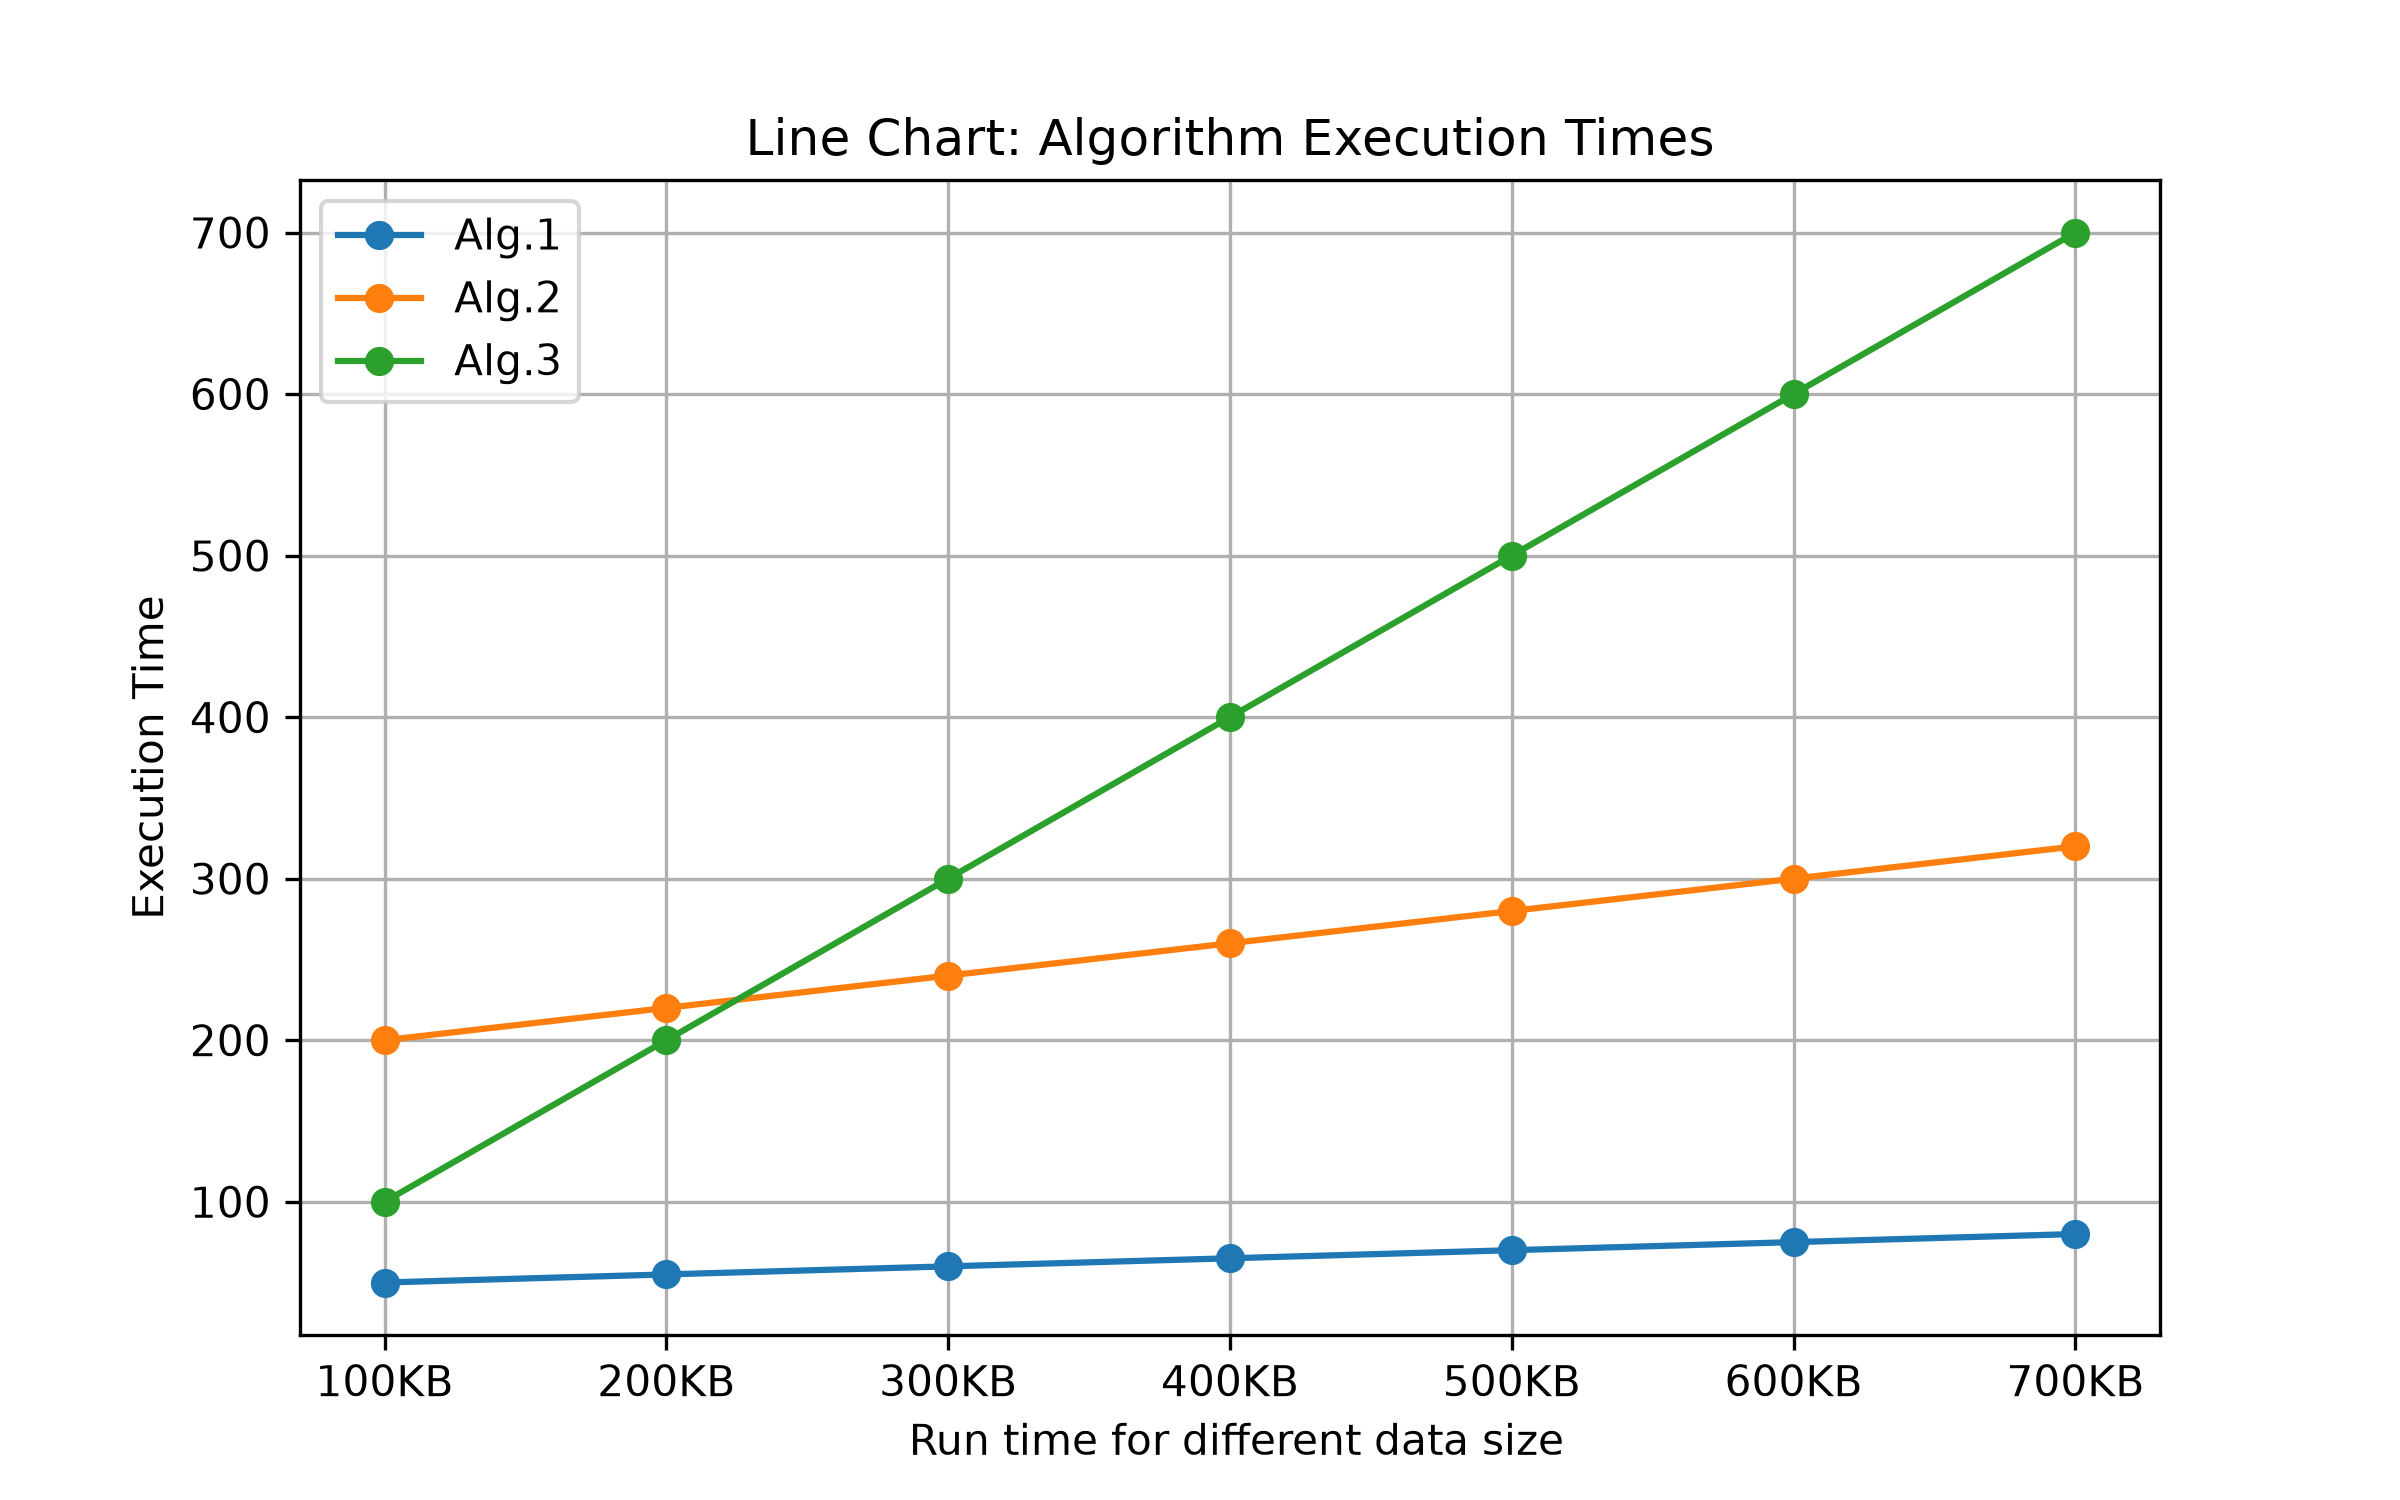
\includegraphics[width=0.9\textwidth]{lin_chart.png}
    \caption{نمودار خطی تغییرات زمان اجرای الگوریتم‌ها بر حسب حجم داده}
\end{figure}

\begin{figure}[H]
    \centering
    \includegraphics[width=0.9\textwidth]{bar_chart.png}
    \caption{نمودار میله‌ای مقایسه‌ای زمان اجرای سه الگوریتم}
\end{figure}

\begin{figure}[H]
    \centering
    \includegraphics[width=0.9\textwidth]{box_chart.png}
    \caption{نمودار جعبه‌ای توزیع داده‌های زمان اجرای هر الگوریتم}
\end{figure}

\subsection{تحلیل نمودارها}
با مشاهده نمودارها می‌توان نتیجه گرفت که با افزایش حجم داده‌ها، زمان اجرای هر سه الگوریتم روند صعودی دارد، اما نرخ رشد آن‌ها کاملاً متفاوت است. الگوریتم ۱ بالاترین کارایی را داشته و کمترین حساسیت را نسبت به افزایش حجم داده نشان می‌دهد (به عنوان مثال، در حجم ۷۰۰ کیلوبایت زمان اجرای آن تنها ۸۰ است). الگوریتم ۲ عملکردی میانی و رشدی متوسط دارد (زمان اجرای ۳۲۰ برای حجم ۷۰۰ کیلوبایت). در مقابل، الگوریتم ۳ با شیب تندی افزایش یافته و بیشترین زمان اجرا را به خود اختصاص می‌دهد (زمان اجرای ۷۰۰ برای ۷۰۰ کیلوبایت). در نتیجه، برای پردازش داده‌های حجیم‌تر، الگوریتم ۱ بهینه‌ترین و الگوریتم ۳ نامناسب‌ترین انتخاب محسوب می‌شود.

\subsection{میانگین زمان اجرای الگوریتم ۲}
با فیلتر کردن سطر مربوط به داده‌های ۷۰۰ کیلوبایت، میانگین زمان اجرای الگوریتم ۲ صرفاً برای حجم داده‌های ۱۰۰ تا ۶۰۰ کیلوبایت از روی فایل اکسل محاسبه شد که مقدار آن برابر است با:
\[ \text{\lr{Average}} = 186.67 \]

\newpage
% ==========================================
\section{انتگرال‌گیری عددی تابع $f(x) = e^{x^2}$}
در این قسمت، مقدار انتگرال معین تابع فوق در بازه $(0,1)$ با روش‌های عددی مختلف محاسبه شده است.

\subsection{کد پایتون پیاده‌سازی}
\begin{latin}
\begin{lstlisting}[language=Python]
import numpy as np
from scipy.integrate import trapezoid, simpson, fixed_quad, quad

def f(x): return np.exp(x**2)
a, b = 0, 1
x_vals = np.linspace(a, b, 101)
y_vals = f(x_vals)

print("Trapezoidal:", trapezoid(y_vals, x_vals))
print("Simpson's:", simpson(y_vals, x=x_vals))
integral_gauss, _ = fixed_quad(f, a, b, n=5)
print("Gaussian:", integral_gauss)
integral_exact, abs_error = quad(f, a, b)
print("Reference:", integral_exact)
\end{lstlisting}
\end{latin}

\subsection{نتایج و تحلیل مقایسه‌ای}
نتایج محاسبات عددی به دست آمده با دقت بالا به شرح زیر است:
\begin{itemize}
    \item \textbf{روش ذوزنقه‌ای (با ۱۰۰ بازه):} $1.46371405$
    \item \textbf{روش سیمپسون (با ۱۰۰ بازه):} $1.46268143$
    \item \textbf{روش انتگرال‌گیری گوسی ($n=5$):} $1.46265172$
    \item \textbf{مقدار دقیق انتگرال (مرجع):} $1.46265175$
\end{itemize}

\textbf{تحلیل و ارزیابی تفصیلی:} \\
تابع $f(x) = e^{x^2}$ به دلیل تقعر رو به بالا و رشد سریع در بازه $(0,1)$، چالش مناسبی برای سنجش روش‌های انتگرال‌گیری است. روش ذوزنقه‌ای به دلیل تقریب زدن تابع با خطوط راست، دارای خطای برش بالاتری است و مقدار انتگرال را بزرگتر از واقعیت محاسبه کرده است. 

روش سیمپسون با تقریب سهموی (درجه ۲) روی بازه‌ها، انحنای تابع را بسیار بهتر پوشش داده و به جواب واقعی نزدیک شده است. در نهایت، روش \textbf{رباعی گوسی} تنها با استفاده از ۵ نقطه ارزیابی، به دلیل انتخاب هوشمندانه نقاط و وزن‌ها، به طور خیره‌کننده‌ای دقیق‌ترین پاسخ را ارائه داده و تا ۷ رقم اعشار با مقدار دقیق مرجع مطابقت دارد. این امر برتری این روش را در توابع هموار نشان می‌دهد.

% ==========================================
\section{مخزن گیت‌هاب}
تمامی کدهای توسعه داده شده در این پروژه به همراه پروژه‌های پیشین در مخزن گیت‌هاب قرار گرفته و کامیت‌های لازم انجام شده است. لینک عمومی مخزن در زیر قرار داده شده است:

\vspace{0.5cm}
\noindent
\href{https://github.com/iamsaad03/MathSoftwareProjects.git}{لینک گیت‌هاب}

\end{document}